%!TEX root = /home/glauffer/Dropbox/FURG/final_project/monografia/monografia.tex
%\chapter{Justificativa e Objetivos}
%por quê???
\chapter{Estrelas Variáveis}
\label{cap:estrelas}

\nocite{Catelan_book}

As estrelas variáveis são uma classificação de estrelas que apresentam alguma varição na sua magnitude aparente. Elas são classificadas devido aos motivos dessa variação em dois grandes grupos: variáveis extrínsecas e variáveis intrínsecas.  A figura \ref{fig:arvore_variab} mostra todas as subclassificações existentes para as estrelas variáveis. Essa família de estrelas possui grande importância, pois são utilizadas como velas padrões e através da relação período-luminosidade são utilizadas para determinar distâncias astronômicas. Ao longo deste capítulo será abordada a classificação desses objetos dando ênfase para as variáveis pulsantes, que são os objetos em estudo deste trabalho, e será visto duas relações importantes envolvendo os períodos de pulsação.%Ao longo desde capítulo será abordada a classificação destes objetos dando ênfase para as variáveis pulsantes, que são os objetos em estudo deste trabalho. Assim como será descrito brevemente os mecanismos de pulsação, teoria sobre as velas padrões e relações matemáticas envolvendo o período. %Ao longo deste capítulo será abordada brevemente a história dessa classe de estrelas assim como a sua classificação.

\begin{figure}[!ht]
\centering
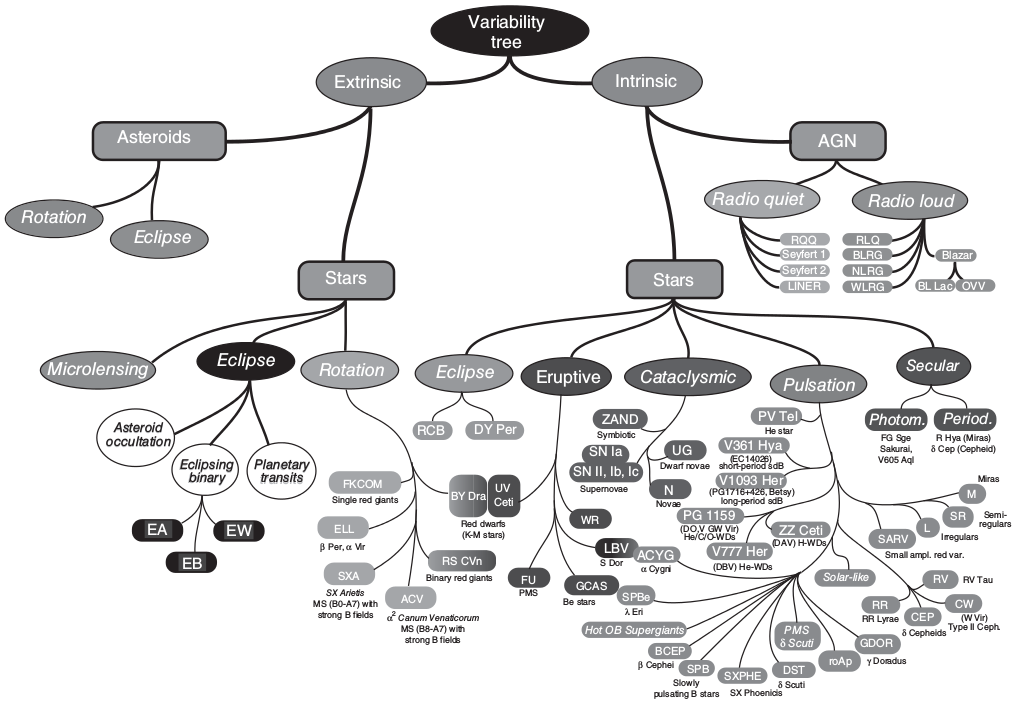
\includegraphics[width=\linewidth]{variability_tree.png}
\caption[Árvore da Variabilidade]{``Árvore da Variabilidade''. A figura mostra todos as possíveis causas de variação no brilho de objetos astronômicos divididas em duas grandes familias, as variáveis Extrínsecas (\textit{Extrinsic}) e as variáveis Intrínsecas (\textit{Intrinsic}). Adaptado de \citet{Catelan_book}.}
\label{fig:arvore_variab}
\end{figure}


%\begin{comment}
%\section{Introdução histórica}
%
%No século 16, acreditava-se que as estrelas eram fixas em posição e com brilho constante. Em 1572, foi observada uma supernova na constelação de Cassiopeia que atingiu magnitude $-4$. Este evento, que foi estudado por Tycho Brahe (1546-1601), fez com que a comunidade astronômica da época voltasse a se interessar pela descobertas de novas estrelas. Alguns anos mais tarde, em 1596, o holandês David Fabricius (1564-1617) fez o primeiro registro de variação em brilho de uma estrela na constelação da Baleia (Cetus).  Essa estrela foi observada em agosto e em outubro havia desaparecido. Em 1603, Johann Bayer observou a mesma estrela e deu o nome de omicron ($O$) Ceti, porém não sabia que era a mesma estrela que Fabricius havia observado, pois achava que se tratava de uma supernova. Em 1638, Johannes Holwarda (1618-1651) observou novamente $O$ Ceti. Em 1662, Johannes Hevelius (1611-1687) fez um estudo detalhado da estrela e a renomeou, a chamando de Mira Ceti (a Maravilhosa). Ismael Bullialdus (1605-1694) percebeu que o pico de magnitude da estrela ocorria sempre um mês mais cedo a cada ano, descobrindo a natureza cíclica de sua variação de brilho. Bullialdus publicou em 1967 que o período de oscilação era de 333 dias. Esta estrela foi a primeira variável a ter o período conhecido e virou referência para as estrelas variáveis de períodos longos, conhecidas hoje em dia como as \textit{variáveis Mira}.
%
%Em 1784, o inglês Jonh Goodricke (1764-1786) descobriu a variação no brilho da estrela $\delta$ Cephei. Ele mediu o período $5\si{\day}8\si{\hour}$. No mesmo ano, o inglês Edward Pigott (1753-1825) descobriu a variabilidade de $\eta$ Aquilae. Ambas essas estrelas se tornaram os protótipos da classe de \textit{variáveis Cefeidas}.
%
%Em 1912, a americana Henrietta Swan Leavitt (1868-1921), derivou uma relação entre o período e a luminosidade (também conhecida como lei de Leavitt) para as estrelas Cefeidas localizadas na Pequena Nuvem de Magalhães \citep{Leavitt1912}. Graças a esta relação que em 1913 Hertzsprung foi capaz de calcular a primeira determinação de distância da Pequena Nuvem \citep{Hertzsprung1913}. Também, utilizando a mesma relação, Hubble determinou a distância de Andrômeda em 1923.
%
%\end{comment}

\section{Variáveis Extrínsecas}

A classificação de variáveis extrínsecas inclui todos os exemplos de estrelas em que a variação da luminosidade é causada por algum processo externo a estrela. Dois exemplos desta classificação são as variáveis eclipsantes e rotacionais.

\subsection{Variáveis eclipsantes}

Esta subclassificação incluí os sistemas binários de estrelas e variações na magnitude devido a asteroides ou exoplanetas. No sistemas binários eclipsantes a variação ocorre devido ao bloqueio da luz causada pela orbita de uma estrela do sistema em torno de sua companheira, ou seja, o movimento de translação de uma estrela em torno da outra faz com que parte da luz seja bloqueada quando as estrelas estão uma atrás da outra em relação ao nosso campo de visão. O período desta variação nos informa o tempo da orbita das estrelas.

Outro motivo externo de variação na magnitude de uma estrela são asteroides ou exoplanetas que estão orbitando alguma estrela. Neste exemplo, a curva de luz é caracterizada por picos de mínimos na magnitude da estrela espaçadas por um valor fixo. Este valor corresponde ao período de translação do exoplaneta ou asteroide.

\begin{figure}[!ht]
\centering
\begin{subfigure}{.5\textwidth}
  \centering
  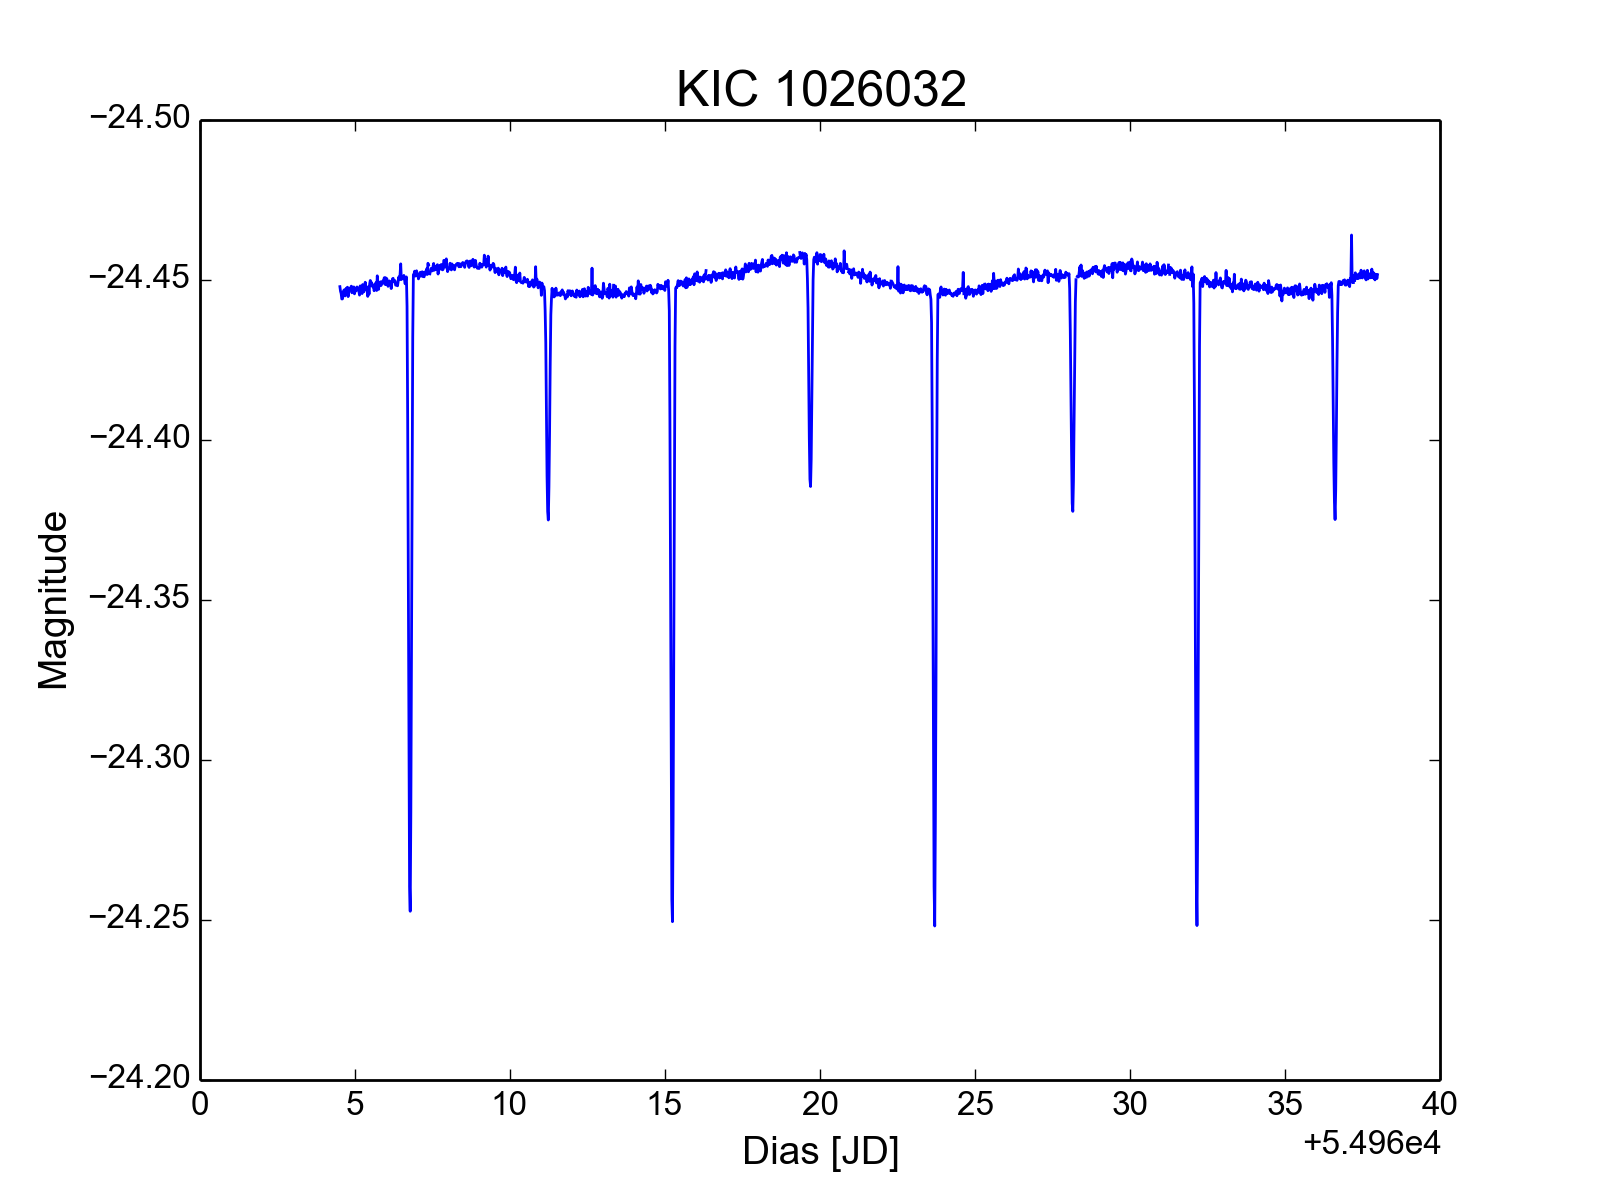
\includegraphics[width=\linewidth]{binary.png}
  \caption{Sistema Binário}
  \label{fig:binaria}
\end{subfigure}%
\begin{subfigure}{.5\textwidth}
  \centering
  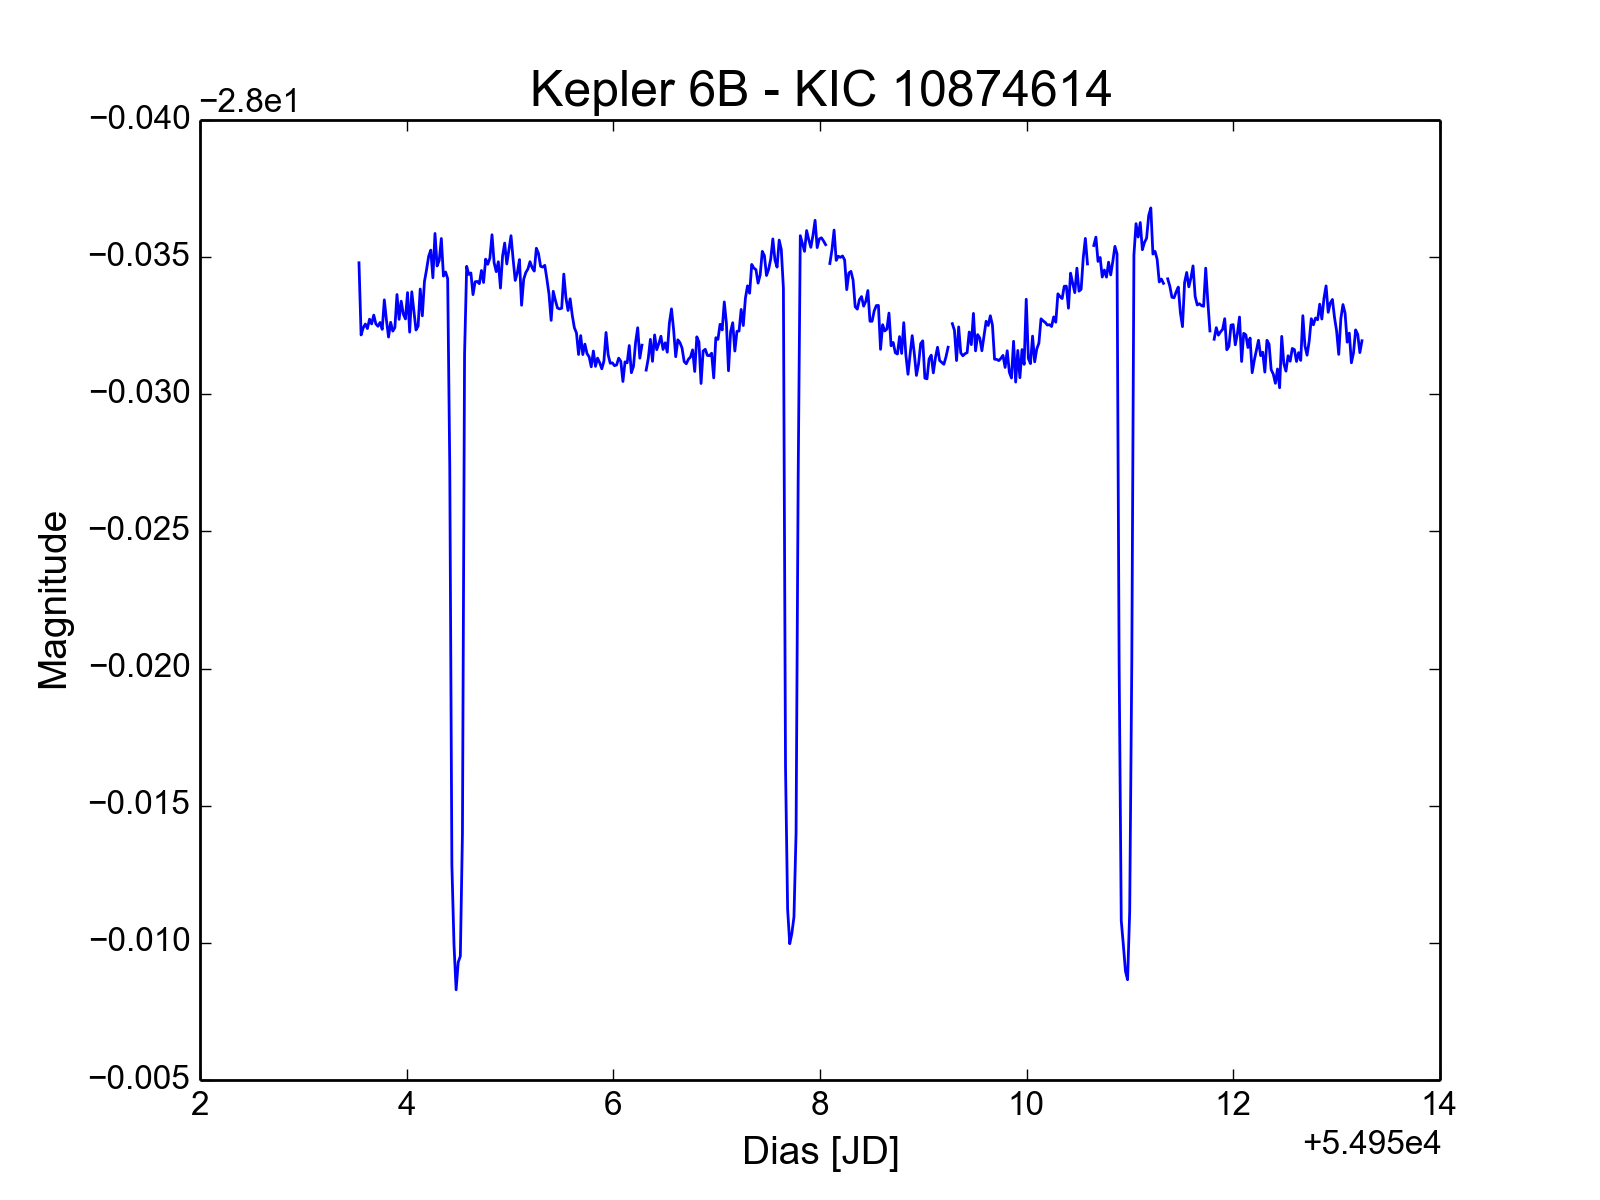
\includegraphics[width=\linewidth]{kepler6b.png}
  \caption{Exoplaneta}
  \label{fig:kepler6b}
\end{subfigure}
\caption[Curva de variáveis eclipsantes.]{Exemplos de curvas de luz de variáveis eclipsantes para dados obtidos do Telescópio Kepler. A imagem (a) é um sistema binário de estrelas. Podemos perceber a os picos de mínimos quando uma estrela bloqueia a luz da outra. A imagem (b) é a curva de luz para o exoplaneta Kepler 6B descoberto em 4 de janeiro de 2010.}
\label{fig:exemplo_eclipsantes}
\end{figure}


\subsection{Variáveis rotacionais}

 Neste caso, a variação ocorre devido a estrela não ser perfeitamente esférica ou possuir manchas em sua superfície. Se a estrela possui um formato mais elíptico e o seu eixo de rotação não está alinhado com o nosso campo de visão, observamos uma oscilação na magnitude devido a variação no raio da estrela. Por outro lado, no caso das manchas na superfície a oscilação ocorre pois estas manchas podem ser ocasionadas por diferença em temperatura ou por um campo magnético local mais intenso, o que interfere na emissão de luminosidade.


\section{Variáveis Intrínsecas}

As variáveis intrínsecas são uma classificação de estrelas em que o motivo da variação da magnitude está relacionada com processos internos da estrela. Essa classificação é dividida em variáveis pulsantes, eruptivas e cataclísmicas.

\subsection{Variáveis eruptivas}

Esta classificação representa estrelas em que ocorrem erupções nas suas cromosferas e coroas devido a atividade magnética, da mesma forma que ocorre ejeções na coroa solar devido ao campo magnético. Essas erupções de massas são chamadas de ventos solares.

\subsection{Variáveis cataclísmicas}

Essa classe de estrelas também é conhecida como \textit{Explosivas} e podem ser subdivididas em quatro categorias: \textit{supernovas}, \textit{novas}, \textit{novas anãs} e \textit{simbióticas}.

As novas e novas anãs são sistemas binários em que a estrela primária seria uma anã branca e a secundária seria uma estrela de baixa massa com tipo espectral M que transfere matéria para a estrela primária. A diferença entre as novas e novas anãs seria o disco de acreção que se forma em torno da novas anãs. Nestes sistemas, a anã branca que normalmente por ser fria não mantém reações termonucleares, começa a receber matéria da sua estrela companheira até um certo ponto em que atinge densidade e temperatura suficientes para queimar o hidrogênio acretado em uma de suas camadas. Este processo é chamado de \textit{nova} e em muitas vezes é recorrente. A curva de luz das novas apresenta um rápido aumento de brilho na ordem de 9 magnitudes seguido de um declínio de 3 a 4 magnitudes em algumas semanas e de uma diminuição lenta que pode durar até 10 anos.

\begin{figure}[ht!]
\centering
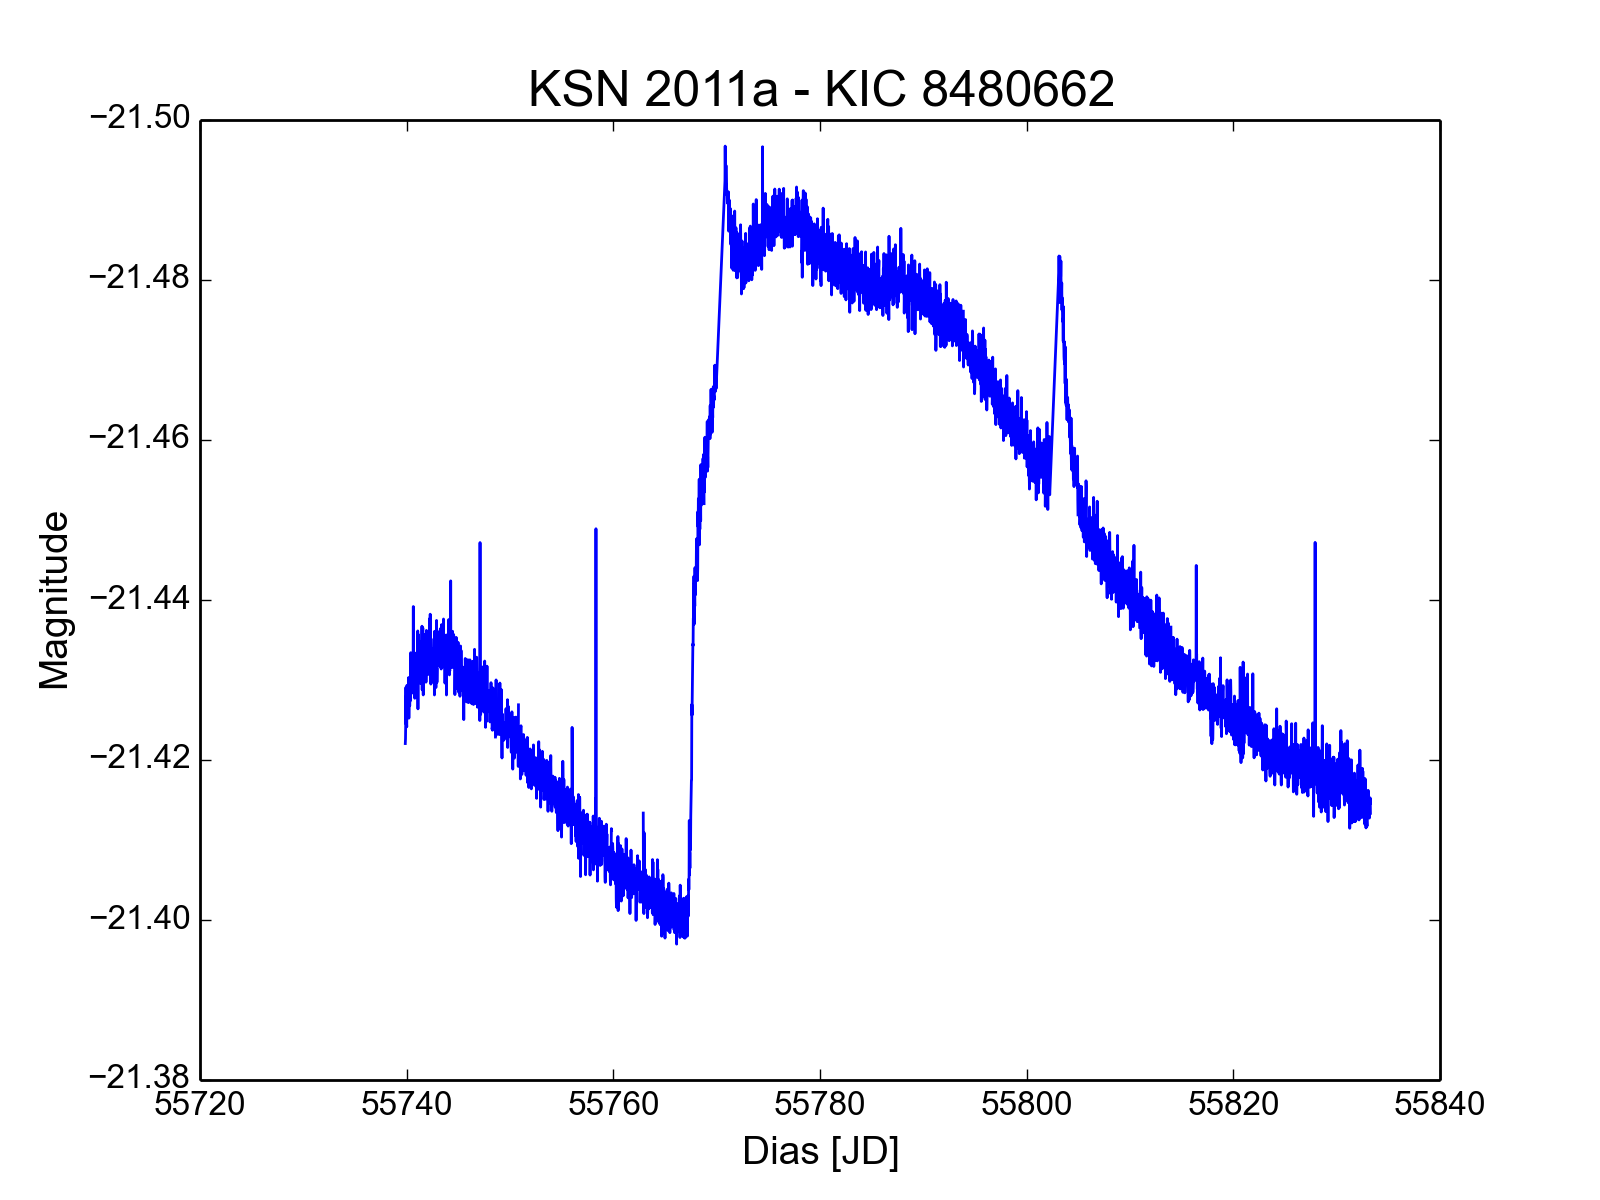
\includegraphics[width=0.5\linewidth]{sn2011a.png}
\caption[Curva de luz da Supernova KSN 2011a]{Curva de luz da Supernova KSN 2011a observada pelo Telescópio Kepler em março de 2016. Há um aumento brusco na magnitude seguido de um decaimento mais lento. Esse aumento é o momento da explosão da estrela.}
\label{fig:exemplo_sn}
\end{figure}

Os sistemas simbióticos são compostos por uma anã branca como estrela primária e uma estrela gigante do tipo espectral M ou N como secundária. Esse sistema possui o comportamento semelhante com as novas e novas anãs, porém ocorrendo em período de tempo maior.

As supernovas são um dos eventos mais energéticos e mais brilhantes que existem no universo. As energias envolvidas na explosão são da ordem de $10^{45} \si{J}$ a $10^{47} \si{J}$ no caso em ocorre colapso do núcleo. Esses eventos são responsáveis pela síntese dos elementos mais pesados do que ferro e são muito utilizados para determinação de distâncias cosmológicas. Um exemplo de curva de luz para a supernova $KSN-2011a$ é mostrado na figura \ref{fig:exemplo_sn}.

\subsection{Variáveis pulsantes}

As variáveis pulsantes são uma classe de estrelas que sofrem pulsações radiais ou não-radiais ou até mesmo esses dois tipos de pulsação. Elas podem ser classificadas entre a forma de pulsação, principal mecanismo que causa a pulsação ou estágio de evoluçao da Estrela. Por exemplo, podemos utilizar a forma de pulsação para classificar as estrelas \textit{Cefeidas}, \textit{RR Lyrae} e \textit{Miras} como as que sofrem pulsação radial. Por outro lado, as estrelas \textit{Beta Cep}, \textit{Gamma Doradus}, \textit{Gamma Virginis} e \textit{ZZ Ceti} são exemplos de estrelas com pulsação não-radial. Por fim, um dos principais exemplo de estrela com os dois tipos de pulsação seria as \textit{Delta Scuti}. Embora existam diversas subclassificações de variáveis pulsantes, será dada ênfase para as denominadas \textit{pulsantes clássicas} em que as Cefeidas e RR Lyrae fazem parte pois estes objetos são os principais alvos do estudo apresentado neste trabalho.

\subsubsection{Cefeidas}

As Cefeidas são estrelas que pulsam de forma radial e estão se deslocando em direção das Gigantes Vermelhas, sendo localizadas na faixa de instabilidade do diagrama H-R. Podem ser divididas em Cefeidas Clássicas e Cefeidas Tipo II. As Clássicas possuem períodos entre $1$ a $100$ dias e são estágios evoluídos de estrelas mais massivas do que o Sol, geralmente possuindo massa entre $2$ a $20$M$_\odot$ e sendo estrelas de população I (maior metalicidade). Por outro lado, as Cefeidas Tipo II são estrelas mais velhas, população II, sendo o estágio mais desenvolvido de estrelas de baixa massa ($0,5$ - $0,6$ M$_\odot$) e possuindo períodos na faixa de $1$ a $25$ dias. Um exemplo de curva de luz para esses dois tipos de Cefeidas pode ser visto na figura \ref{fig:exemplo_cep}.

\begin{figure}[h!]
\centering
\begin{subfigure}{.5\textwidth}
  \centering
  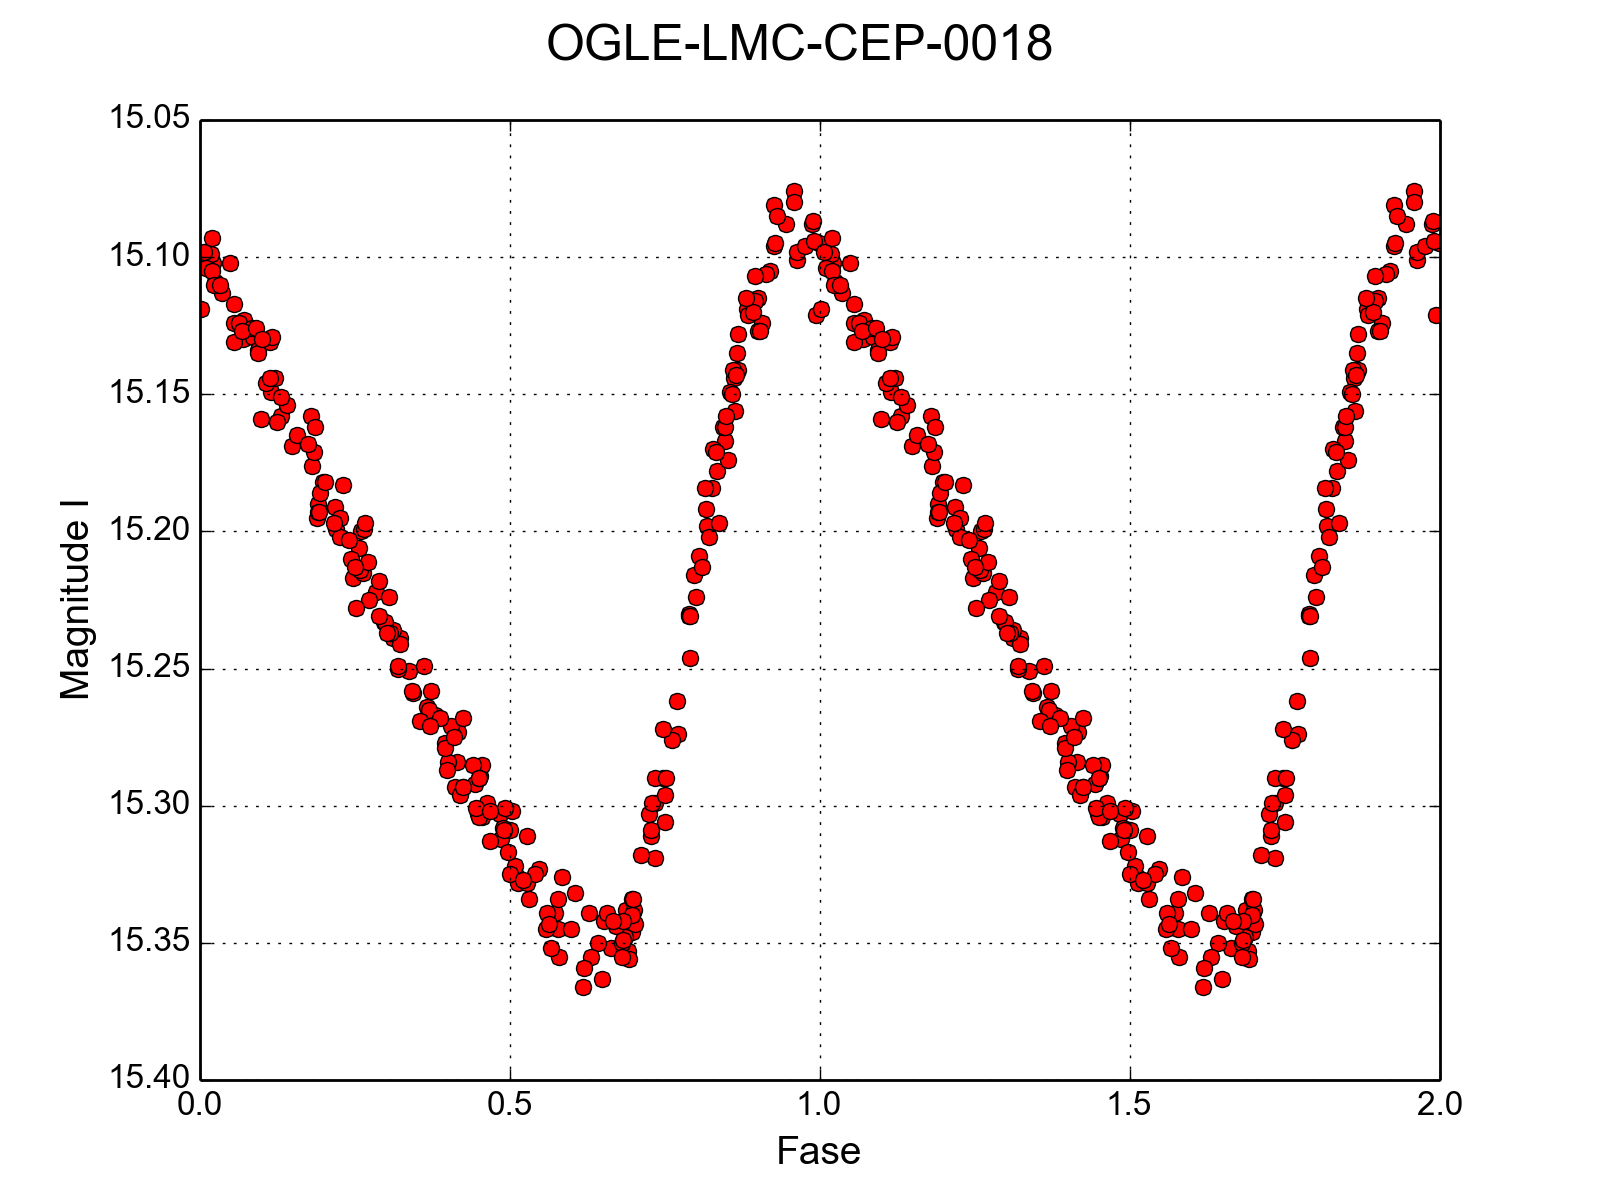
\includegraphics[width=\linewidth]{0018_correct.png}
  \caption{Cefeida Clássica}
 % \label{fig:right}
\end{subfigure}%
\begin{subfigure}{.5\textwidth}
  \centering
  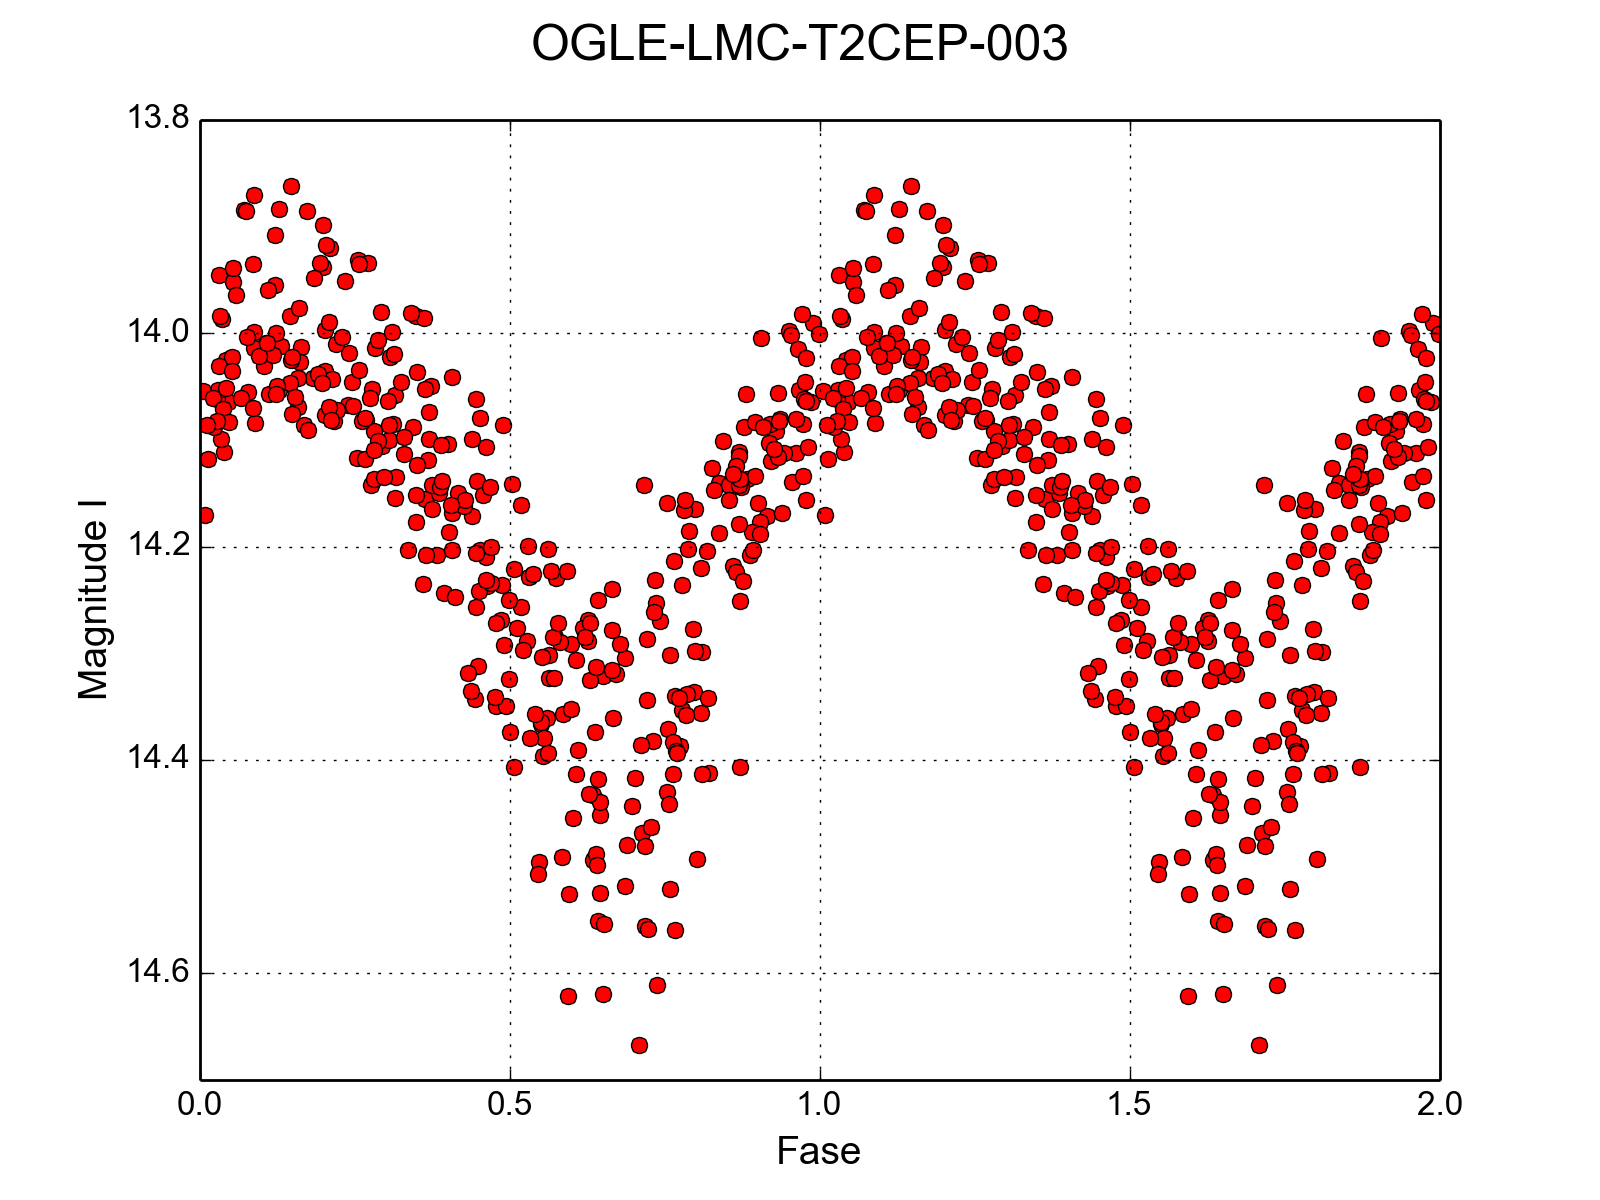
\includegraphics[width=\linewidth]{type2Cep.png}
  \caption{Cefeida tipo II}
 % \label{fig:wrong}
\end{subfigure}
\caption[Curva de luz de Cefeidas]{Exemplos de curvas de luz no espaço de fase para uma  Cefeida clássica (a) e uma tipo II (b) do catálogo OGLE. O espaço de fase da imagem na esquerda foi construído utilizando o período $P=4,0478$ e na imagem da direita foi utilizado o período $P=35,6599$.}
\label{fig:exemplo_cep}
\end{figure}

As cefeidas podem ser subdivididas de acordo com o seu modo de pulsação. As estrelas que pulsam no modo radial fundamental são denominadas FU (do inglês \textit{Fundamental Mode}) e as que pulsam no primeiro sobre tom do modo radial são chamadas de FO (do inglês \textit{First Overtone}).

A grande importância deste tipo de estrela está na descoberta da relação entre período e luminosidade derivada por Henrietta Leavitt \citep{Leavitt1912} que possibilitou a determinação de distâncias astronômicas em uma escala superior do que a paralaxe trigonométrica, que era a técnica utilizada na época.


\subsubsection{RR Lyrae}

As RR Lyrae são uma das estrelas utilizadas para determinação de distâncias e determinação de propriedades de populações estelares mais antigas. No diagrama H-R elas são localizadas dentro da faixa de instabilidade e possuem magnitude absoluta em torno de $+0,6$ (na faixa do visível), temperaturas em entre $6000$ e $7250 \si{K}$ e massa entre $0,6$ e $0,8$ M$_\odot$. Essas estrelas possuem períodos entre $0,2$ e $1,0$ dias e são encontradas em sistemas com idades superiores a $10$ giga-ano, sendo ótimas velas padrões para determinação de distância de sistemas mais antigos.

\begin{figure}[!ht]
\centering
\begin{subfigure}{.5\textwidth}
  \centering
  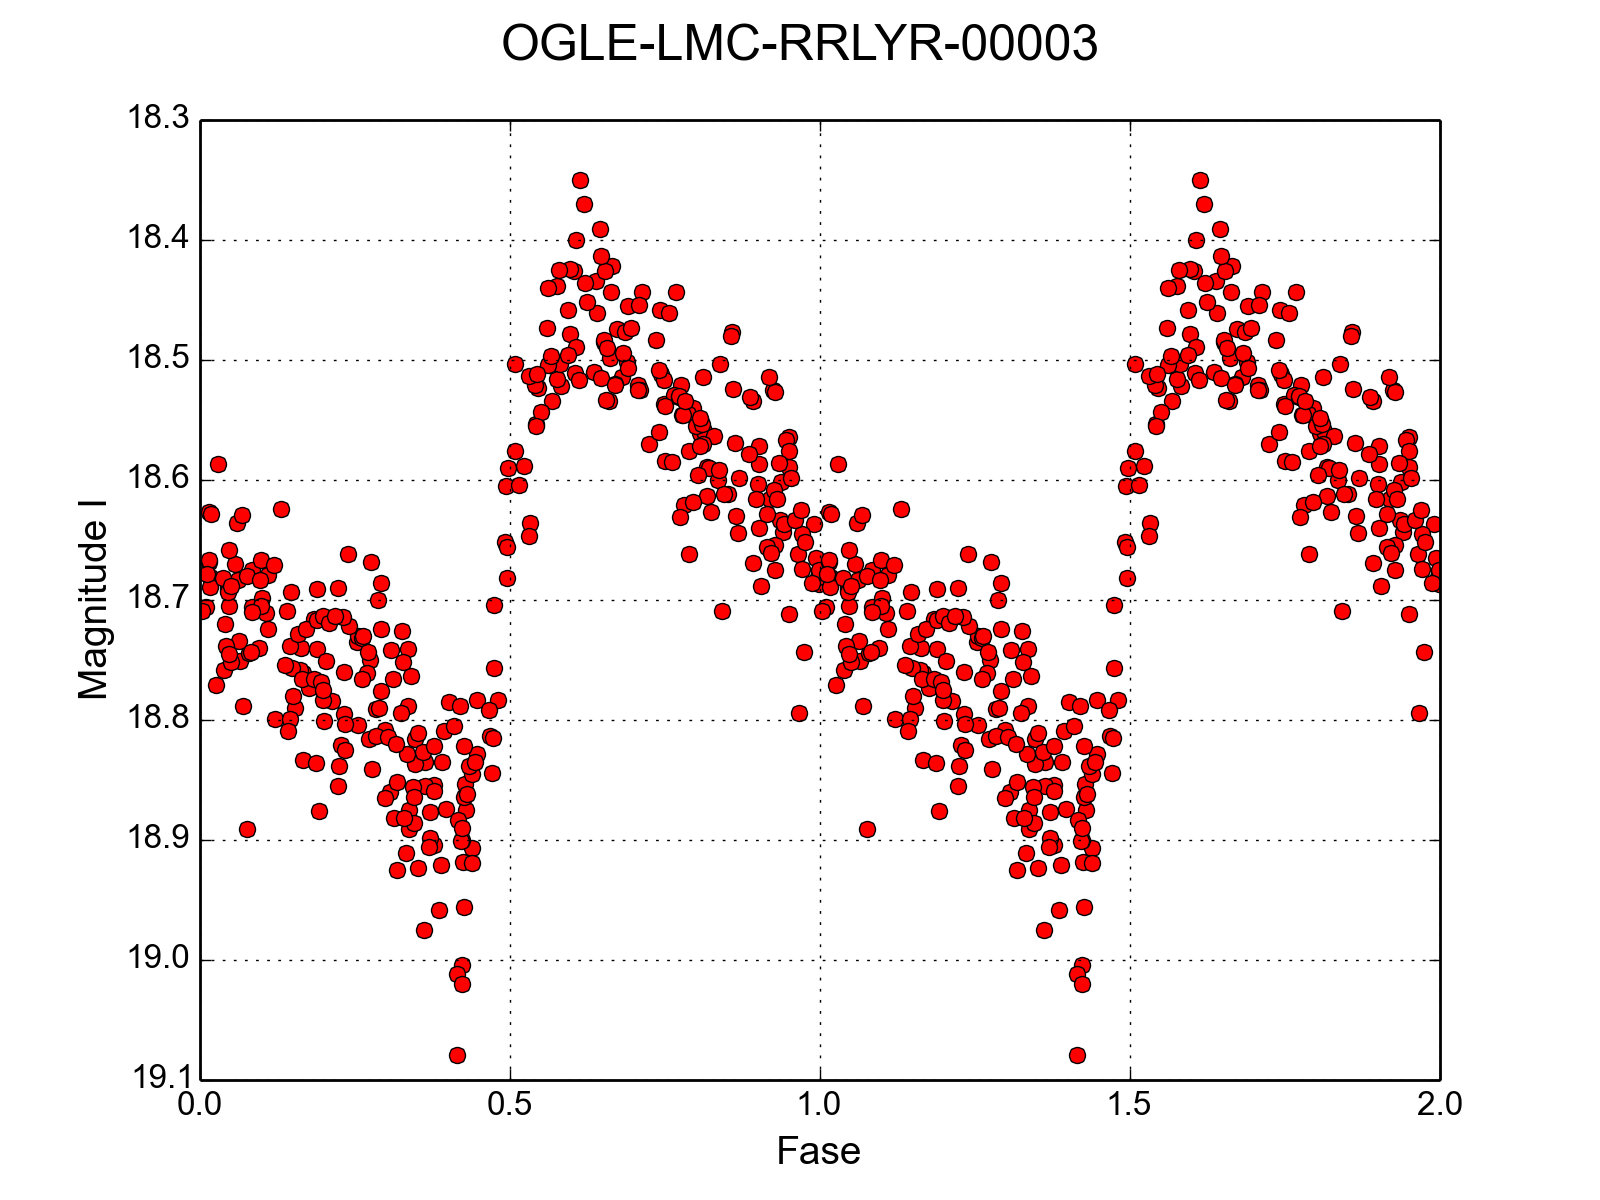
\includegraphics[width=\linewidth]{rrlyrAB.png}
  \caption{RR Lyrae AB}
  %\label{fig:right}
\end{subfigure}%
\begin{subfigure}{.5\textwidth}
  \centering
  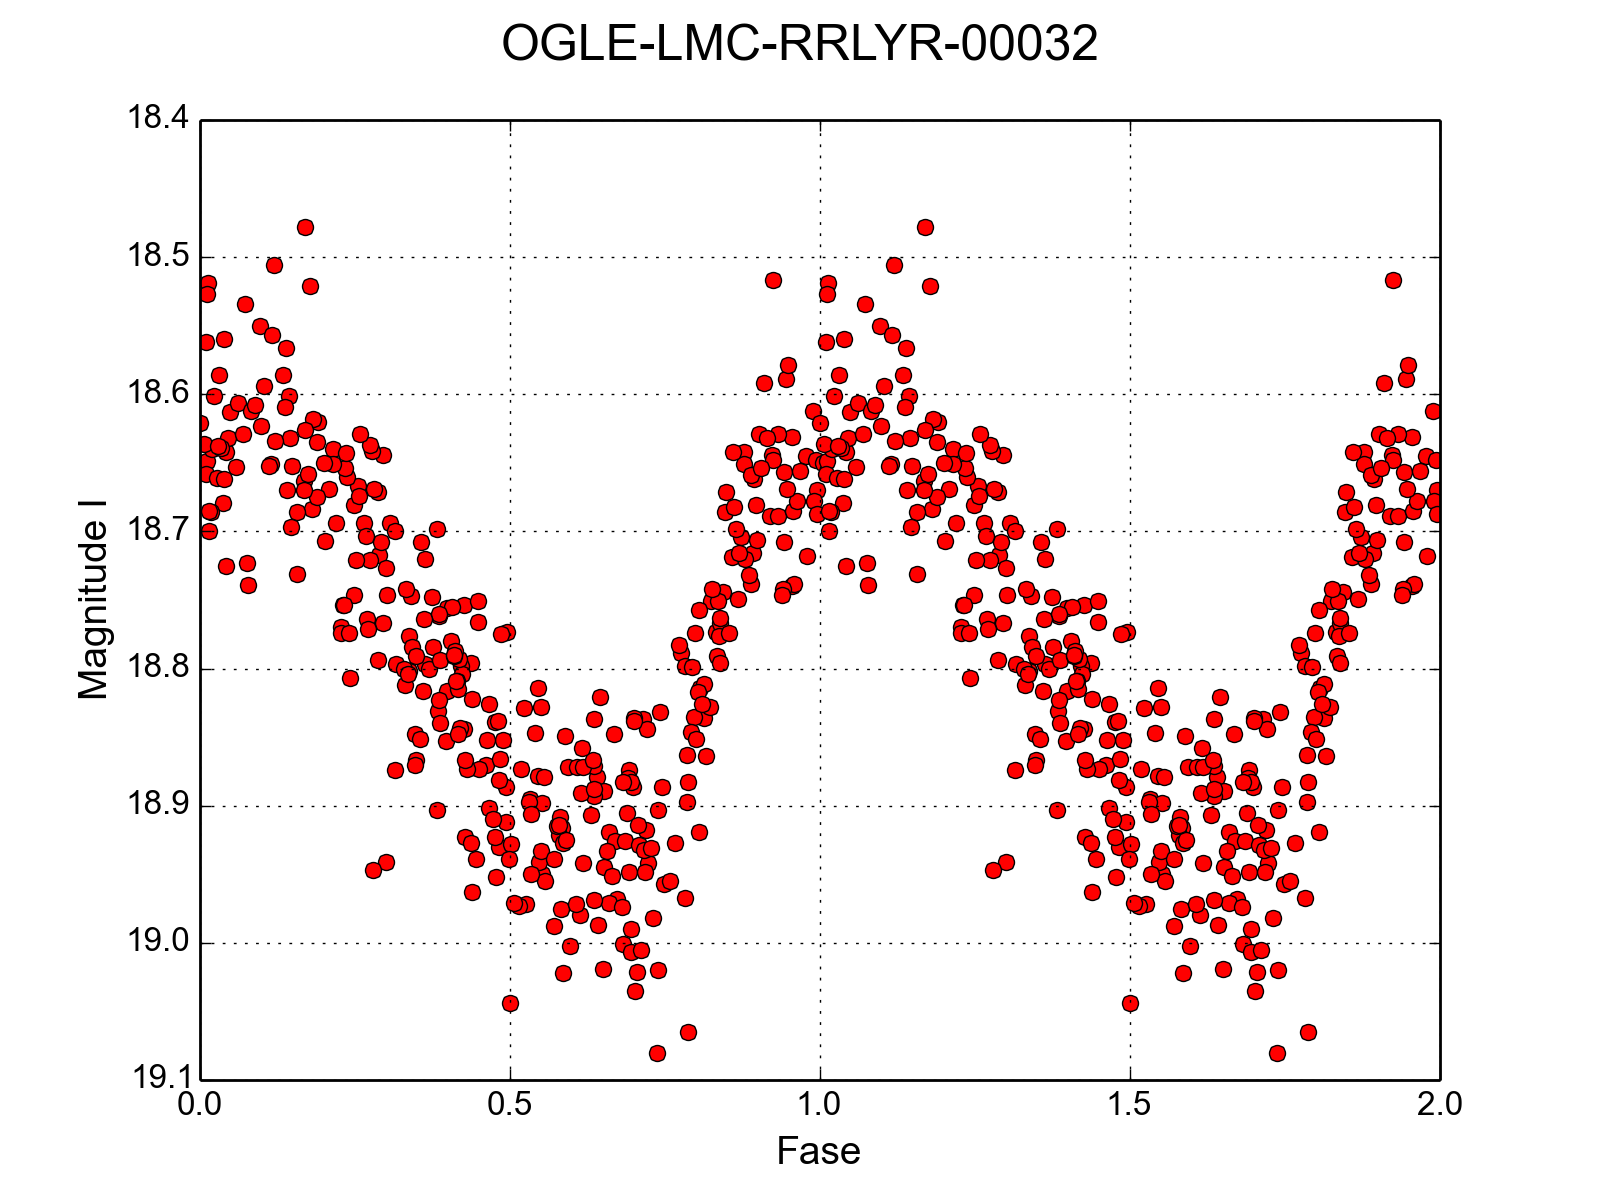
\includegraphics[width=\linewidth]{rrlyrC.png}
  \caption{RR Lyrae C}
  %\label{fig:wrong}
\end{subfigure}
\caption[Curva de luz de RR Lyrae]{Exemplos de curvas de luz no espaço de fase para uma  RR Lyrae tipo $AB$ (a) e uma tipo $C$ (b) do catálogo OGLE. O espaço de fase da imagem na esquerda foi construído utilizando o período $P=0,6565$ e na imagem da direita foi utilizado o período $P=0,3535$.}
\label{fig:exemplo_rrlyr}
\end{figure}


Essas estrelas são classificadas como tipos $AB$ ou $C$ dependendo da sua forma de pulsação o que modifica o formato da sua curva de luz. As RR Lyrae do tipo $AB$ pulsam no modo radial fundamental, enquanto que as do tipo $C$ pulsam no primeiro sobre tom do modo radial. Um exemplo de curva de luz pode ser visto na figura \ref{fig:exemplo_rrlyr}.


Como a figura \ref{fig:exemplo_rrlyr} mostra, a curva de luz das RR Lyrae do tipo $AB$ possuem um aumento brusco da luminosidade seguido de um decaimento mais lento. Por outro lado, as RR Lyraes do tipo $C$ apresentam um comportamento mais senoidal.

\section{Relações com o Período}

\subsection{Período - Luminosidade (\textit{Lei de Leavitt})}

A relação entre o período e a luminosidade foi descoberta por Henrietta Leavitt, que  era uma astrônoma que trabalhava no observatório de Harvard catalogando estrelas em placas fotométricas. Em 1912, ela derivou uma relação entre a luminosidade e o período de pulsação de $25$ estrelas na Pequena Nuvem de Magalhães, estrelas que mais tarde foram identificadas como Cefeidas. Essa relação possui a forma
\begin{align}
m = a + b \log P \label{eq:leavitt_law}
\end{align}
em que $m$ é a magnitude aparente, $P$ é o período de pulsação e $a$ e $b$ são constantes. Essas constantes podem ser obtidas pelo método dos mínimos quadrados.

Como as $25$ estrelas analisadas pela Henrietta pertenciam a Pequena Nuvem de Magalhães, ela inferiu que essas estrelas possuiam as mesmas propriedades e assim a relação entre a magnitude aparente e o período implicaria na relação entre a magnitude absoluta e o período da seguinte forma,
\begin{align}
M = a^\prime + b \log P
\end{align}
em que $M$ é a magnitude absoluta e $a^\prime$ é a constante $a$ deslocada por um determinado valor. Esse valor que desloca a constante foi identificado mais tarde como modulo de distância. Desta forma, obtendo as constantes $a$ e $b$ e tendo calculado o período, podemos estimar o valor da magnitude absoluta e obter as distâncias das estrelas. Essa relação ficou conhecida como \textit{Lei de Leavitt} ou relação Período - Luminosidade.

\subsection{Período - Densidade}

As oscilações radiais são  causadas pelas ondas sonoras que ressoam no interior da estrela. Podemos estimar o valor do período de pulsação $ \Pi$ apenas considerando quanto tempo uma onda sonora deveria levar para atravessar o diâmetro total de uma estrela de raio $R$ e densidade constante $\rho$, ou seja
\begin{align}
\Pi = \frac{4 R}{v_s} . \label{eq:periodo_densidade}
\end{align}
Para isto, vamos partir da equação da velocidade do som em um gás adiabático,
\begin{align}
v_s^2 = \frac{\gamma P}{\rho}
\end{align}
em que $P$ é a pressão e $\gamma$ é a razão entre os calores específicos à pressão constantes e à volume constante,
\begin{align}
\gamma = \frac{C_P}{C_V}.
\end{align}
Para um gás monoatômico, $\gamma = 5/3$, e a pressão pode ser calculada através da condição do equilíbrio hidrostático,  %306
\begin{align}
\frac{dP}{dr} = - G\frac{M \rho}{r^2}
\end{align}
em que $M$ é a massa dentro da esfera de raio $r$ e $G$ é a constante gravitacional. Considerando uma esfera perfeita, podemos reescrever a massa como
\begin{align}
M = \dfrac{4}{3}\pi r^3 \rho .
\end{align}
Substituindo na equação da pressão,
\begin{align}
\frac{dP}{dr} = - \frac{4}{3}\pi G \rho^2 r
\end{align}
e fazendo a separação de variáveis e integrando a pressão de $ 0$ a $P$ (pois a pressão na camada mais externa é zero) e o raio de $r$ a $R$ ficamos com,
\begin{align}
P(r) = \frac{2}{3}\pi G \rho^2 (R^2 - r^2)
\end{align}
agora, substituindo a pressão na equação da velocidade do som,
\begin{align}
v_s^2 = \frac{\gamma P}{\rho} = \frac{2}{3}\gamma \pi G \rho (R^2 - r^2)
\end{align}
obtemos uma relação para a velocidade do som no interior da estrela. Por fim, substituindo essa relação de velocidade na equação \eqref{eq:periodo_densidade} e integrando de $0$ a $R$,
\begin{align}
\Pi \approx 2 \int_0^R \frac{dr}{v_s} \approx 2 \int_0^R \frac{dr}{\sqrt{\frac{2}{3}\gamma \pi G \rho (R^2 - r^2)}}
\end{align}
a integral é multiplicada por dois para considerar todo o diâmetro da estrela. Desta forma, obtemos que o período de pulsação é igual a
\begin{align}
\Pi \approx \sqrt{\frac{3\pi}{2\gamma G \rho}} \text{.}
\end{align}

Esse resultado, chamado de relação Período-Densidade, nos mostra que período de pulsação é inversamente proporcional à raiz quadrada da densidade média da estrela, ou seja, estrelas mais densas possuem períodos de pulsação menores do que estrelas menos densas. Por exemplo, para uma estrela com densidade igual a do sol, $\rho = 1409 \si{kg} \, \si{m}^{-3}$ \citep{keplerLivro2013}, e considerando $\gamma = 1$ por simplicidade e $G= 6,67 \times 10^{-11} \si{m}^3 \si{kg}^{-1} \si{s}^{-2}$, obtemos:
\begin{align}
\Pi \approx  7081,12 \si{s}.
\end{align}

